\documentclass[aps,prl,twocolumn,superscriptaddress,nofootinbib]{revtex4-2}

\usepackage{fontspec}
\usepackage{xeCJK}
\usepackage{amsmath,amssymb}
\usepackage{graphicx}
\usepackage{booktabs}
\usepackage{siunitx}
\usepackage{hyperref}
\usepackage{xcolor}

\setCJKmainfont{Noto Serif CJK SC}
\setCJKsansfont{Noto Sans CJK SC}
\setCJKmonofont{Noto Sans Mono CJK SC}

\graphicspath{
  {./}
  {data_analysis/week_1/results/}
  {data_analysis/week_2/results/}
  {data_analysis/combined_analysis/results/}
}

\begin{document}

\title{宇宙线穿过铅板后的有效符合率衰减研究}

\author{学生姓名}
\affiliation{实验课程 / 实验室名称，学校名称}

\date{\today}

\begin{abstract}
本文分析了一个基于上下双闪烁体探测器的宇宙线铅板阻挡实验。实验将不同厚度的铅板置于两个探测器之间，并使用固定阈值条件 $(\mathrm{area}>30)\land(\mathrm{area2}>30)$ 选取双探测器符合事件。第一周数据覆盖 0--30 片铅板，符合率随铅板厚度增加整体下降，并可用有效指数衰减模型描述。第二周数据覆盖 0、40、50、60 片铅板，但其 0 片基准、下探测器脉冲积分分布和条件符合比均与第一周存在显著差异，表明存在探测器响应漂移。通过 0 片基准缩放可得到 0--60 片铅板的综合趋势，但厚铅板区间仍非单调，说明单一缩放因子不能完全修正跨周系统效应。因此，本实验测得的是在固定几何、固定阈值和实际探测效率条件下的有效符合率衰减，而不是宇宙线 $\mu$ 子在铅中的纯吸收长度。
\end{abstract}

\maketitle

\section{引言}

宇宙线是来自地球大气层外的高能粒子流。原初宇宙线主要由质子、氦核和更重的原子核组成。当这些高能粒子进入大气层后，会与大气中的氮、氧等原子核发生强相互作用，产生强子簇射。簇射中产生的 $\pi$ 介子和 $K$ 介子进一步衰变，形成大量次级 $\mu$ 子。由于 $\mu$ 子质量较大、能量通常达到 GeV 量级，并且存在相对论时间膨胀效应，因此许多 $\mu$ 子能够到达海平面并被实验室探测器记录。

在近地面实验中，宇宙线 $\mu$ 子具有两个重要特点。第一，通量随时间存在统计涨落，也可能受气压、温度和探测器工作状态影响。第二，实验室探测到的并不是单一能量、单一方向的粒子束，而是具有连续能谱和角分布的粒子集合。因此，简单教学实验中测得的计数率变化通常是探测器接受度、粒子能量损失、多重散射和阈值效率共同作用的结果。本文后续使用“有效”一词，正是为了避免把实验计数率直接解释成某个单一微观过程的概率。

海平面附近宇宙线 $\mu$ 子的角分布常近似写为
\begin{equation}
I(\theta)\simeq I(0)\cos^2\theta ,
\end{equation}
其中 $\theta$ 为相对竖直方向的天顶角。因此，上下排列的两个闪烁体探测器可视为一个简单的几何望远镜，主要接收接近竖直方向的宇宙线事件。

在双探测器构型中，只有同时穿过上、下闪烁体并在两个通道中产生足够大信号的粒子才会被计入符合事件。这个选择条件能显著抑制单个探测器中的噪声、暗计数和偶然触发，但也会引入更强的几何限制。若铅板使粒子发生散射，即使粒子本身没有被吸收，也可能因为偏离下探测器而不再满足符合条件。因此，双探测器实验对“穿过铅板后的方向保持能力”非常敏感。

本实验的目标是测量宇宙线穿过不同厚度铅板后，双探测器符合率如何变化。需要强调的是，符合率下降并不等同于 $\mu$ 子被铅板直接吸收。铅板可能导致低能成分被削弱，也可能通过多重散射使粒子偏离下探测器，从而降低几何符合效率。因此本文使用“有效符合率衰减”描述实验观测量。

铅作为高原子序数、高密度材料，常用于辐射屏蔽和吸收体实验。对于电磁辐射和低能带电粒子，铅的屏蔽效果非常明显；对于海平面宇宙线中的 GeV 量级 $\mu$ 子，铅的直接吸收能力则相对有限。因此，在几十毫米铅厚范围内，若观测到符合率下降，更合理的解释通常不是大量 $\mu$ 子被完全阻止，而是低能成分、散射偏转和探测器阈值共同改变了可记录事件的比例。

这也是本实验与普通“遮挡光线”实验的区别。铅板不是简单地把所有入射粒子按固定比例挡住，而是改变穿过材料后粒子的能量、方向和可探测信号。由于探测器只对超过阈值的脉冲积分作出有效记录，材料效应会通过电子学阈值被进一步放大或压缩。实验结论必须围绕“探测器记录到什么”展开，而不是只围绕“粒子在材料中发生了什么”展开。

从实验报告的角度看，本文关注三个问题。第一，同一周内部的计数率是否随铅板厚度表现出可解释的下降趋势。第二，两周数据是否具有相同的探测器响应基准，能否直接合并。第三，如果不能直接合并，是否可以通过 0 片铅板基准进行经验缩放，并在缩放后讨论 0--60 片铅板范围内的整体趋势。

该问题具有典型的实验物理训练意义。理论上，宇宙线与物质相互作用可以由粒子输运、能量损失和散射理论描述；实验上，实际观测量却是电子学系统输出的波形积分和触发计数。二者之间需要通过探测器效率、阈值选择和几何接受度连接。因此，本实验不是单纯把计数画成曲线，而是需要判断哪些变化来自物理吸收体，哪些变化来自探测系统本身。这样的区分是小型核与粒子物理实验中最关键的分析步骤之一。

本文的写作结构如下。首先介绍双探测器符合测量的物理原理和误差定义；随后分别分析第一周和第二周数据，避免在探测条件不一致时过早合并；接着利用 0 片铅板数据检查跨周一致性，并通过基准缩放构造综合曲线；最后讨论该综合曲线的可信范围、系统误差来源以及后续改进方向。

\section{实验原理}

实验记录上、下两个探测器的脉冲积分量，分别记为 $\mathrm{area}$ 和 $\mathrm{area2}$。本文统一采用固定阈值：
\begin{equation}
\mathrm{area}>30,\qquad \mathrm{area2}>30 .
\end{equation}
双探测器符合事件定义为
\begin{equation}
\mathrm{coincidence}=(\mathrm{area}>30)\land(\mathrm{area2}>30).
\end{equation}
相应计数定义为
\begin{align}
N_{\rm up} &= \#(\mathrm{area}>30),\\
N_{\rm down} &= \#(\mathrm{area2}>30),\\
N_{\rm coin} &= \#[(\mathrm{area}>30)\land(\mathrm{area2}>30)].
\end{align}

固定阈值的优点是分析规则清楚，并且能够保证不同铅板厚度下使用同一套事件选择标准。本文没有使用 25、30、35 等多阈值扫描，而是只保留 $\mathrm{area}>30$ 与 $\mathrm{area2}>30$ 作为唯一判断标准。这样做使得符合数、透过率和阻挡率之间的比较更加直接，但代价是结果会更明显地受到探测器增益漂移的影响。若某一周下探测器整体信号变小，固定阈值会使该周的有效探测效率降低。

双探测器符合率为
\begin{equation}
R_{\rm coin}=\frac{N_{\rm coin}}{T}.
\end{equation}
本实验每个 run 的测量时间取 $T=\SI{3600}{s}$，时间不确定度取 $\sigma_T=\SI{60}{s}$。计数服从泊松统计，因此符合率相对误差写为
\begin{equation}
\frac{\sigma_R}{R_{\rm coin}}
=\sqrt{\frac{1}{N_{\rm coin}}+\left(\frac{\sigma_T}{T}\right)^2}.
\end{equation}

这里的计数率应理解为单位时间内满足双阈值符合条件的事件数。若用 counts/hour 表示，则在本实验假设下数值上等于一小时测量得到的 $N_{\rm coin}$。由于测量时间存在约 1 min 的不确定度，时间误差约占 $1/60\simeq1.7\%$。对于 $N_{\rm coin}\sim10^3$ 的数据，泊松相对误差约为 $2\%$ 左右，因此两类误差量级相近，均应纳入拟合权重和结果解释。

为讨论铅板阻挡能力，定义相对透过率
\begin{equation}
\mathcal{T}(x)=\frac{R_{\rm coin}(x)}{R_{\rm coin}(0)},
\end{equation}
以及有效阻挡率
\begin{equation}
\mathcal{B}(x)=1-\mathcal{T}(x).
\end{equation}
这里的 $\mathcal{B}$ 只表示在本实验几何和阈值条件下有效符合率降低的比例，并不是 $\mu$ 子真实吸收概率。

相对透过率的物理意义是把同一周的 0 片铅板数据作为本底基准，观察加入铅板后符合率剩余的比例。该量可以削弱同一周内总通量归一化的不确定性，例如当天宇宙线通量、整体采集时间或触发规模的变化。然而，如果 0 片基准本身来自不同周，且探测器响应已经改变，则不同周的 $\mathcal{T}$ 仍不能简单视为同一个物理曲线上的点。

此外，本文还使用条件符合比
\begin{equation}
\frac{N_{\rm coin}}{N_{\rm up}},
\end{equation}
其物理意义为：已经被上探测器记录到的候选事件中，有多少比例也能被下探测器记录到。该量可部分减小总触发规模变化带来的影响，但仍然受到下探测器效率和阈值响应影响。

如果把上探测器看作入射候选粒子的抽样器，把下探测器看作穿过铅板和几何路径后的确认器，那么 $N_{\rm coin}/N_{\rm up}$ 可近似写成
\begin{equation}
\frac{N_{\rm coin}}{N_{\rm up}}
\sim \epsilon_{\rm down}\, A_{\rm geom}\, P_{\rm pass}(x),
\end{equation}
其中 $\epsilon_{\rm down}$ 表示下探测器有效探测效率，$A_{\rm geom}$ 表示几何接受度因素，$P_{\rm pass}(x)$ 表示粒子经过厚度 $x$ 后仍能满足符合条件的概率。这个表达式只是概念分解，但它说明同一个观测量中混合了探测器效率、几何和材料作用。若 $\epsilon_{\rm down}$ 在两周之间变化，则即使 $P_{\rm pass}(x)$ 相同，条件符合比也会改变。

偶然符合也是双探测器实验中需要关注的量。若上下通道单独计数率分别为 $R_{\rm up}$ 和 $R_{\rm down}$，符合时间窗宽度为 $\Delta t$，则偶然符合率量级可估为
\begin{equation}
R_{\rm acc}\sim R_{\rm up}R_{\rm down}\Delta t .
\end{equation}
当前分析主要基于已经处理好的符合事件和脉冲积分阈值，没有单独展开偶然符合修正。由于宇宙线符合实验中真实穿越事件通常可通过时间相关性筛选，偶然符合应作为后续精细分析的潜在系统项列入误差预算。

铅板对宇宙线的影响主要来自两类机制。其一是电离能损，带电粒子在铅中传播时与原子电子相互作用并损失能量。对于 GeV 量级 $\mu$ 子，铅中几十毫米厚度通常不足以造成完全吸收，但会影响低能尾部成分。其二是库仑多重散射，粒子通过高 $Z$ 材料时会发生小角度累积偏转。多重散射角的近似尺度可写为
\begin{equation}
\theta_0\simeq \frac{13.6\ {\rm MeV}}{\beta pc}z
\sqrt{\frac{x}{X_0}}
\left[1+0.038\ln\left(\frac{x}{X_0}\right)\right],
\end{equation}
其中 $X_0$ 为材料辐射长度，$p$ 为粒子动量，$z$ 为电荷数。虽然该公式主要用于估算散射角分布宽度，但它说明厚铅板会增强方向偏转，从而降低上下探测器的几何符合概率。

由于宇宙线 $\mu$ 子能谱较宽，本实验中不同能量粒子对铅板的响应并不相同。高能 $\mu$ 子更容易穿透铅板并保持方向，低能粒子则更容易在能损和散射后不再形成有效符合。因此，随着铅板厚度增加，探测器记录到的事件集合可能逐渐偏向较高能、较小散射角的粒子。这种“样本组成变化”也会使简单指数模型只能作为经验近似，而不是完整输运方程的严格解。

还需要区分单通道计数和双通道符合计数。单通道计数主要反映该探测器自身的触发效率、噪声和入射粒子规模；双通道符合计数同时要求上下两个通道满足阈值，并且对粒子轨迹有更强约束。因此，在判断铅板阻挡能力时，$N_{\rm coin}$ 比单通道计数更能代表穿过整个装置的有效宇宙线事件，但也更容易受任一通道效率变化影响。

\section{数据与处理方法}

实验数据分两周采集。第一周包含 0、10、20、30 片铅板，对应厚度 0、5、10、\SI{15}{mm}。第二周包含 0、40、50、60 片铅板，对应厚度 0、20、25、\SI{30}{mm}。每片铅板厚度为 \SI{0.5}{mm}。

原始 ROOT 文件通过 \texttt{uproot} 读取，并预处理为轻量化 NumPy 文件。后续分析只使用事件级标量分支，包括 \texttt{area}、\texttt{area2}、\texttt{amp}、\texttt{base}、\texttt{rms} 和 \texttt{Index\_minamp}。第一周和第二周分别先独立分析，随后再进行跨周一致性检查。

预处理阶段的目标不是改变数据，而是把后续分析所需的关键信息从 ROOT 文件中提取出来，保存为更易读取的 \texttt{npz} 文件。这样可以避免每次绘图和拟合时重复解析 ROOT 文件，也便于对每个 run 的基础统计量进行统一管理。分析脚本进一步输出符合数、单通道通过数、条件符合比、脉冲积分分布图、能谱相关直方图和拟合结果。

本文采用“先分周、后合并”的分析策略。这样安排的原因是两周测量条件并不完全相同。若直接把第一周 0--30 片和第二周 40--60 片拼接成一条曲线，隐含假设是两周探测器效率、阈值响应、通道增益和几何位置完全一致。但从 0 片基准对比可见该假设不成立。因此，第一步必须分别判断每周内部的趋势，再讨论跨周归一化是否合理。

为定量描述衰减趋势，使用两个经验指数模型。第一个模型拟合归一化透过率：
\begin{equation}
\mathcal{T}(x)=\exp(-x/\lambda_{\rm eff}).
\end{equation}
第二个模型拟合绝对符合率：
\begin{equation}
R_{\rm coin}(x)=R_0\exp(-x/\lambda_{\rm eff}).
\end{equation}
其中 $\lambda_{\rm eff}$ 是有效衰减长度，包含多重散射、几何接受度、探测效率和阈值响应等因素，不能解释为 $\mu$ 子在铅中的纯吸收长度。

采用指数模型的理由是它提供了一个简单、可比较的单参数尺度。当厚度范围不大且衰减不强时，指数函数在局部会接近一条直线，这也是拟合图中曲线看起来较直的原因。若对模型取对数，
\begin{equation}
\ln \mathcal{T}(x)=-x/\lambda_{\rm eff},
\end{equation}
则理想指数衰减在半对数坐标下为直线。不过本文图中的拟合是在原始透过率或 counts/hour 上完成的，直线外观主要来自衰减幅度较小，而不是把所有图都改画成了对数化直线。

拟合时的误差估计采用计数泊松误差和时间误差的合成形式。对于透过率 $\mathcal{T}=R(x)/R(0)$，原则上还应考虑 0 片基准点的不确定度传播。由于本文目标是给出课程实验层面的初步分析，拟合主要用于比较趋势和获得有效尺度，而不是追求材料常数的高精度测量。报告中所有 $\lambda_{\rm eff}$ 的解释都应服从这一限制。

除拟合外，能谱与脉冲积分分布也是重要诊断工具。这里的“能谱”并不是严格校准后的粒子能量谱，而是探测器脉冲积分量的分布。对于闪烁体探测器，脉冲积分与沉积能量、光收集效率、SiPM 增益和电子学响应有关。若同一通道在两周中的脉冲积分分布发生整体移动，则说明固定阈值对应的物理探测效率发生变化，不能仅用宇宙线通量变化解释。

在数据处理上，本文把每个 run 的分析结果分为三类。第一类是计数类结果，包括上通道通过数、下通道通过数和双通道符合数。第二类是归一化结果，包括透过率、阻挡率和条件符合比。第三类是分布类结果，包括 \texttt{area} 与 \texttt{area2} 的直方图、脉冲积分比较图以及用于诊断响应漂移的 0 片对比图。三类结果相互补充：计数类结果给出实验主观测量，归一化结果用于比较厚度变化，分布类结果用于判断计数变化是否可信。

本文没有对原始波形重新进行峰值寻找或积分窗口优化，而是使用已有数据分支中的脉冲积分量。这使分析流程更简洁，也减少了人为调参空间。但这种做法要求原始数据中的积分定义在不同 run 之间保持一致。若采集程序或通道设置发生变化，\texttt{area} 和 \texttt{area2} 的分布会发生系统移动，固定阈值分析就会受到影响。第二周数据正体现了这种风险。

为了保持分析透明性，所有关键判断都尽量使用可直接复现的量。例如，跨周差异不是只通过拟合参数判断，而是同时比较 0 片符合数、\texttt{area2} 均值和条件符合比。只有当多个独立观测量指向同一结论时，才把第二周问题解释为探测器响应变化。这样的交叉检查比单纯依赖拟合优度更稳健。

\section{物理图像与模型适用范围}

本实验的核心物理图像可以用“入射粒子束、吸收体、几何望远镜”三部分理解。宇宙线粒子从上方进入实验装置，先经过上探测器，再穿过不同厚度的铅板，最后到达下探测器。若上下两个探测器都记录到超过阈值的脉冲积分，则该事件被计为双探测器符合。铅板厚度增加后，符合率可能下降，说明能完整通过这一实验链条的事件比例降低。

这个图像中最容易误解的一点是“穿透”和“符合”并不等价。一个 $\mu$ 子即使穿过了铅板，也可能因为散射角增大而错过下探测器；也可能因为沉积能量较小，使下探测器脉冲积分低于阈值；还可能由于电子学响应漂移，使同样的沉积能量在不同时间对应不同的 \texttt{area2} 数值。因此，实验记录的不是单纯穿透概率，而是穿透、几何保持和探测响应的乘积。

在理想情况下，如果探测器效率稳定、几何位置固定、宇宙线通量稳定，且吸收体只引入一个随厚度指数下降的有效通过概率，则符合率可写为
\begin{equation}
R_{\rm coin}(x)=\Phi\, A\, \epsilon_{\rm up}\epsilon_{\rm down}
P_{\rm eff}(x),
\end{equation}
其中 $\Phi$ 表示入射宇宙线通量，$A$ 表示几何接受度，$\epsilon_{\rm up}$ 与 $\epsilon_{\rm down}$ 表示上下探测器效率，$P_{\rm eff}(x)$ 表示铅板厚度为 $x$ 时仍能形成有效符合的概率。若进一步假设 $P_{\rm eff}(x)=\exp(-x/\lambda_{\rm eff})$，就得到本文使用的经验指数模型。

这个分解也说明了为什么同一周归一化透过率较有意义。对于同一周内部数据，若 $\Phi$、$A$、$\epsilon_{\rm up}$ 和 $\epsilon_{\rm down}$ 近似不随厚度改变，则
\begin{equation}
\mathcal{T}(x)=\frac{R_{\rm coin}(x)}{R_{\rm coin}(0)}
\simeq \frac{P_{\rm eff}(x)}{P_{\rm eff}(0)} .
\end{equation}
当 0 片时取 $P_{\rm eff}(0)=1$，透过率就近似反映铅板造成的有效符合概率变化。这正是第一周数据可以独立解释的原因。

相反，跨周比较时，上式中的 $\epsilon_{\rm down}$ 很可能已经变化。若第一周和第二周下探测器效率分别为 $\epsilon_{\rm down}^{\rm W1}$ 和 $\epsilon_{\rm down}^{\rm W2}$，则绝对符合率之比不仅包含铅板厚度效应，也包含效率比
\begin{equation}
\frac{\epsilon_{\rm down}^{\rm W2}}{\epsilon_{\rm down}^{\rm W1}} .
\end{equation}
因此，第二周 40--60 片数据不能直接接到第一周 0--30 片数据之后。必须先检查 0 片基准和脉冲积分分布，确认效率差异的存在。

有效指数模型的另一个限制来自宇宙线能谱。海平面 $\mu$ 子不是单能粒子，低能粒子和高能粒子在铅中的行为不同。如果用 $E$ 表示粒子能量，则更一般的符合率可以形式上写成
\begin{equation}
R_{\rm coin}(x)=\int dE\, d\Omega\,
\Phi(E,\Omega)\, A(E,\Omega)\,
\epsilon(E,\Omega)\, P(E,\Omega,x).
\end{equation}
本文的指数模型相当于把这个复杂积分压缩成一个有效参数 $\lambda_{\rm eff}$。因此，$\lambda_{\rm eff}$ 是实验装置和样本平均后的量，而不是铅材料本身的唯一属性。

在铅板较薄、衰减幅度较小时，指数模型和线性近似在数值上很接近。对 $x/\lambda_{\rm eff}\ll1$，有
\begin{equation}
\exp(-x/\lambda_{\rm eff})
\simeq 1-\frac{x}{\lambda_{\rm eff}} .
\end{equation}
第一周最大厚度为 \SI{15}{mm}，而拟合得到的 $\lambda_{\rm eff}$ 为 $10^2$ mm 量级，因此拟合曲线在图中看起来接近直线是合理的。这种外观不表示物理模型就是线性模型，也不表示拟合一定是在对数坐标完成。

对于厚铅板区间，多重散射效应可能更明显。若粒子动量较低，散射角增大后更容易偏离下探测器有效面积，使符合率下降。与此同时，宇宙线样本中较高能粒子更容易保留在符合样本中，因此厚铅板后的事件组成可能发生改变。由于本实验没有动量选择和角度重建，无法单独提取这些物理过程，只能通过有效符合率总体反映。

本文暂不把 Rossi 曲线作为主要分析对象。Rossi 曲线通常需要研究宇宙线在吸收体中产生二次粒子所导致的计数率先增加后减少现象。要可靠讨论该曲线，需要稳定探测器条件、更多吸收体厚度点以及对二次粒子贡献的专门分析。当前两周数据首先暴露的是探测效率变化问题，因此更适合讨论有效符合率衰减和跨周归一化，而不是完整 Rossi 曲线。

综上，本文采用的模型属于“最小可解释模型”：它足够简单，可以用少量数据点拟合和比较；同时又明确承认 $\lambda_{\rm eff}$ 的有效性质，不把它误认为严格材料常数。这种处理方式适合课程实验报告，也符合当前数据质量所允许的解释范围。

\section{第一周结果}

第一周数据的固定阈值符合计数如表~\ref{tab:week1} 所示。随着铅板数从 0 增加到 30 片，符合数从 3357 降至 3046，相对透过率降至约 0.907。

\begin{table}[h]
\caption{第一周固定阈值符合统计。}
\label{tab:week1}
\begin{ruledtabular}
\begin{tabular}{cccc}
Run & 铅板数 & $N_{\rm coin}$ & $\mathcal{T}$\\
\hline
5181 & 0  & 3357 & 1.000\\
5182 & 10 & 3136 & 0.934\\
5183 & 20 & 3119 & 0.929\\
5184 & 30 & 3046 & 0.907\\
\end{tabular}
\end{ruledtabular}
\end{table}

从表中可以看出，第一周数据的主要特征是整体下降但下降幅度较小。0 到 10 片铅板的变化较明显，而 10 到 20 片之间变化很小，20 到 30 片继续下降。这种现象在宇宙线实验中并不罕见，因为样本同时受到统计涨落、角分布、粒子能谱和探测器响应的影响。只要整体趋势与误差范围内的模型相容，就可以把它作为有效阻挡趋势讨论。

\begin{figure}[h]
\centering
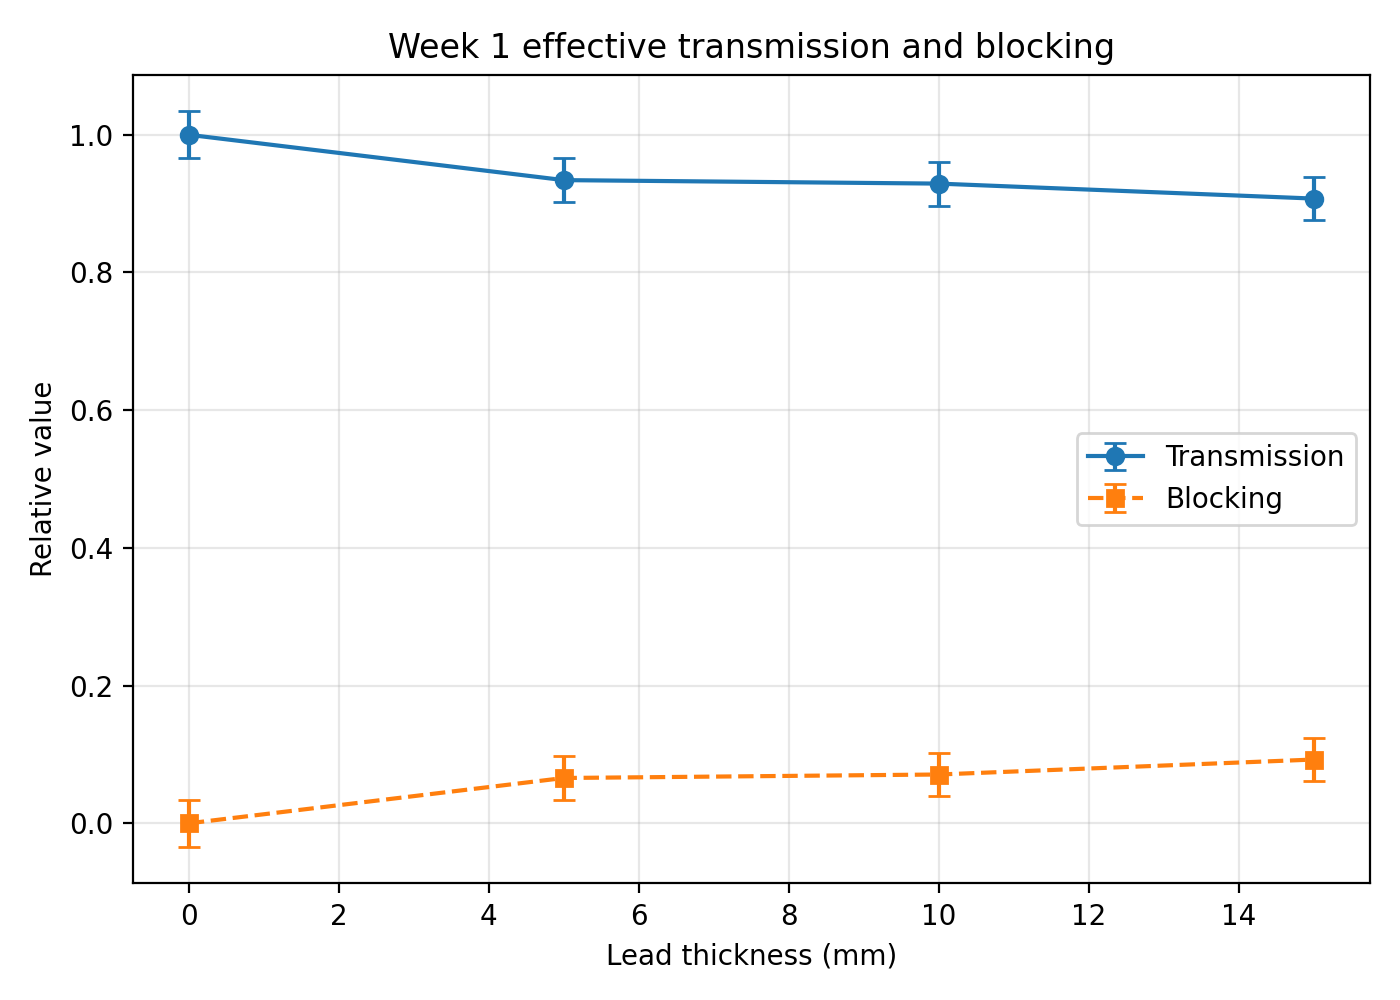
\includegraphics[width=\linewidth]{figures/week1_transmission_blocking.png}
\caption{第一周有效透过率和有效阻挡率随铅板厚度的变化。}
\label{fig:week1_transmission}
\end{figure}

对第一周数据进行指数拟合，透过率模型给出
\begin{equation}
\lambda_{\rm eff}=(137.45\pm34.85)\ \mathrm{mm},
\end{equation}
对应 $\chi^2/{\rm ndf}=0.335$。绝对符合率模型给出
\begin{equation}
\lambda_{\rm eff}=(168.09\pm62.02)\ \mathrm{mm},
\end{equation}
对应 $\chi^2/{\rm ndf}=0.701$。两种拟合均说明第一周内部趋势较稳定。

透过率拟合和绝对符合率拟合的 $\lambda_{\rm eff}$ 并不完全相同，这是因为二者处理归一化和误差传播的方式不同。透过率模型把 0 片点固定为归一化基准，更强调相对变化；绝对符合率模型同时拟合 $R_0$ 和衰减长度，更直接保留 counts/hour 的物理量纲。两者给出的有效衰减长度都在 $10^2$ mm 量级，说明第一周数据在有限厚度范围内给出了相互一致的衰减尺度。

\begin{figure}[h]
\centering
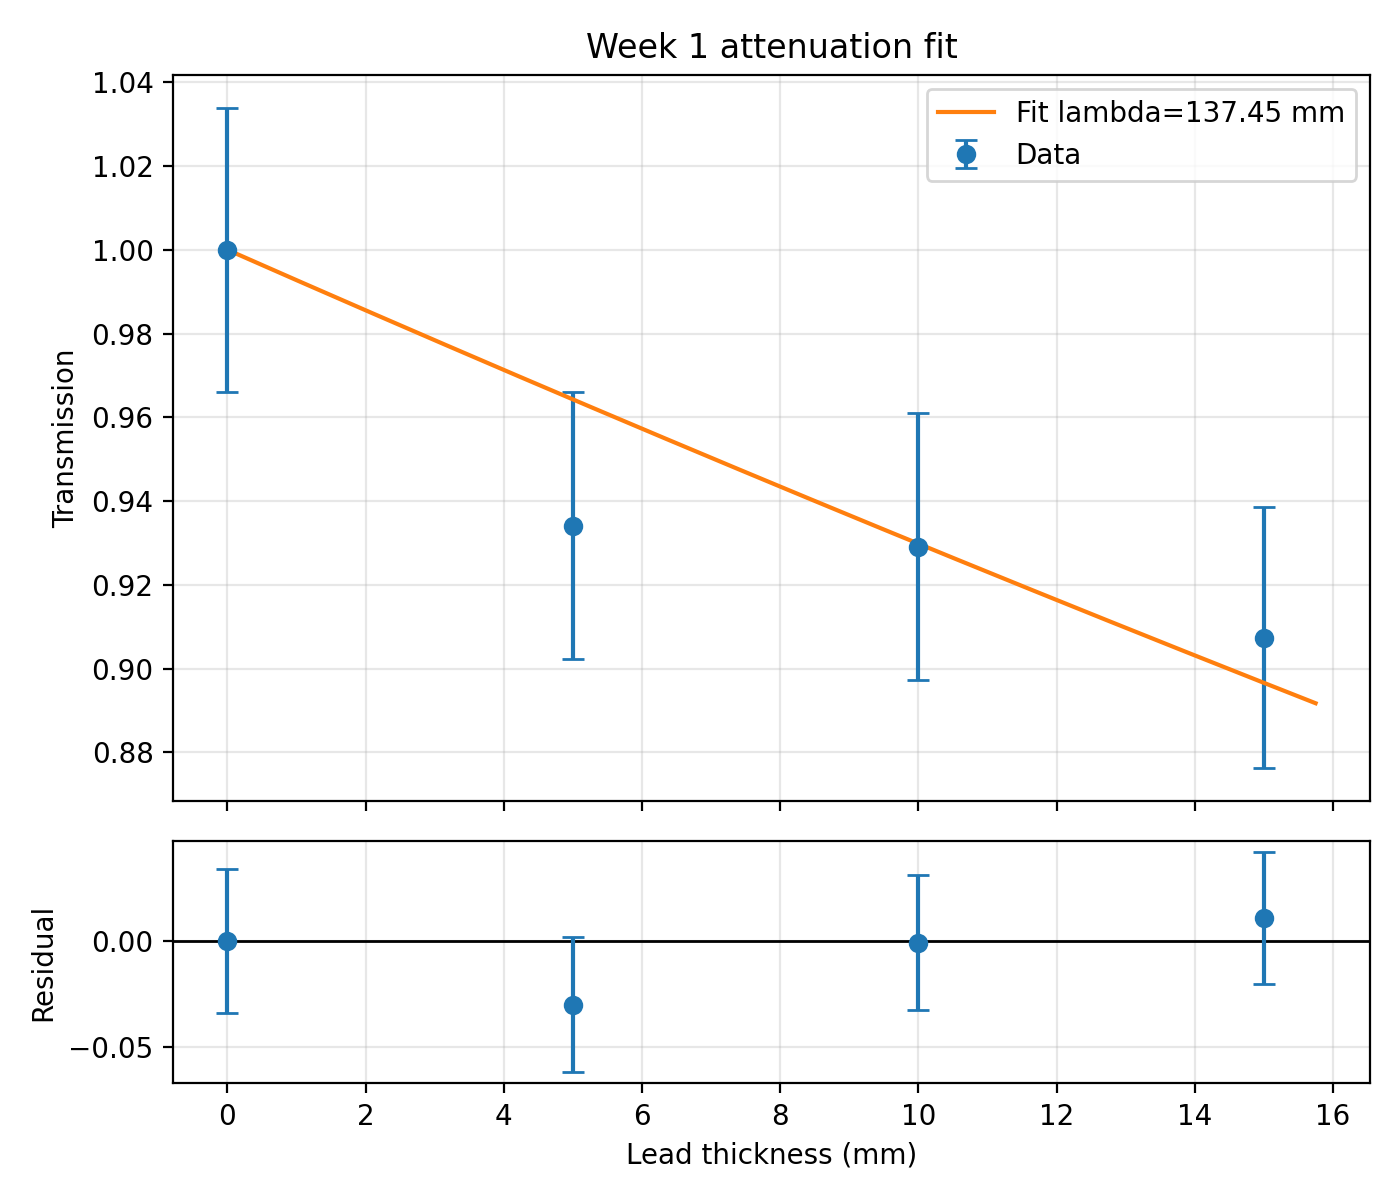
\includegraphics[width=\linewidth]{fit/week1_attenuation_fit.png}
\caption{第一周归一化透过率的指数拟合。由于铅厚范围相对于 $\lambda_{\rm eff}$ 较小，指数曲线在该范围内近似线性。}
\label{fig:week1_fit}
\end{figure}

第一周的物理解释可以概括为：铅板增加后，能够保持足够信号并通过上下探测器符合条件的事件比例降低。该降低可能来自低能粒子成分减少，也可能来自散射导致的几何损失。由于本实验没有测量单个粒子的动量和入射角，不能进一步把这两种贡献分开。因此，本节结果最适合作为固定装置条件下的经验衰减测量。

从有效阻挡率角度看，第一周 30 片铅板对应的阻挡率约为 $1-0.907\simeq0.093$，即在 \SI{15}{mm} 铅厚下，约 $9\%$ 的原本 0 片基准符合事件不再满足双探测器符合条件。这个数值不应理解为 \SI{15}{mm} 铅吸收了 $9\%$ 的海平面 $\mu$ 子，而应理解为本装置在该阈值和几何条件下损失了约 $9\%$ 的有效符合事件。

第一周数据也说明，在较薄铅板范围内，宇宙线符合率变化并不剧烈。这与海平面 $\mu$ 子较强的穿透能力相符。若实验希望更明显地区分不同厚度的影响，可以增加测量时间、重复测量每个厚度点，或增加更厚的吸收体范围。但增加厚度后，多重散射和探测器效率问题会更加突出，因此仍需保持探测器状态稳定。

第一周拟合优度较小还应谨慎理解。$\chi^2/{\rm ndf}$ 小于 1 可能说明模型与数据相容，也可能说明误差估计偏保守或数据点数量较少。第一周只有四个厚度点，拟合自由度有限，因此不应过度强调拟合曲线的精确性。更合理的表述是：第一周数据没有显示与单调有效衰减模型相冲突的明显异常。

若从 counts/hour 的角度观察，第一周每个点都对应一小时测量，因此符合数本身就是每小时符合计数。0 片到 30 片的下降约为 311 counts/hour。与泊松误差和时间误差相比，这一总下降量具有可观察意义，但单个相邻厚度点之间的差异可能并不总是显著。因此第一周结论应基于整体趋势，而不是把 10 片和 20 片之间的微小差别解释为具体物理结构。

\section{第二周结果}

第二周数据覆盖厚铅板区间，其固定阈值符合计数如表~\ref{tab:week2} 所示。与第一周不同，第二周 40、50、60 片铅板点并不呈现单调下降趋势。

\begin{table}[h]
\caption{第二周固定阈值符合统计。}
\label{tab:week2}
\begin{ruledtabular}
\begin{tabular}{cccc}
Run & 铅板数 & $N_{\rm coin}$ & $\mathcal{T}$\\
\hline
51811 & 0  & 1831 & 1.000\\
5185  & 40 & 1523 & 0.832\\
5186  & 50 & 1579 & 0.862\\
5187  & 60 & 1687 & 0.921\\
\end{tabular}
\end{ruledtabular}
\end{table}

如果只从铅板厚度的物理直觉出发，更厚的铅板通常应导致有效符合率不增加，至少在统计平均意义上应呈现下降或接近平台的趋势。但第二周数据中，40 片点最低，随后 50 片和 60 片反而上升。这说明第二周厚铅板数据不能仅用铅板阻挡解释，必须考虑探测器状态变化、采集条件变化或统计与系统误差共同作用。

第二周透过率拟合得到
\begin{equation}
\lambda_{\rm eff}=(188.23\pm33.90)\ \mathrm{mm},
\end{equation}
对应 $\chi^2/{\rm ndf}=2.384$。绝对符合率拟合得到
\begin{equation}
\lambda_{\rm eff}=(239.47\pm75.59)\ \mathrm{mm},
\end{equation}
对应 $\chi^2/{\rm ndf}=6.364$。较大的 $\chi^2/{\rm ndf}$ 表明第二周数据存在明显系统效应，不能作为干净的单调衰减曲线解释。

第二周仍然进行指数拟合，是为了和第一周保持相同的分析流程，而不是因为该模型已经充分描述了数据。尤其是 counts/hour 拟合的 $\chi^2/{\rm ndf}$ 明显偏大，表明各点相对于单调指数曲线的偏离已经超过统计误差能够自然解释的范围。因此，第二周拟合参数只能看作经验比较量，不能作为可靠材料参数使用。

\begin{figure}[h]
\centering
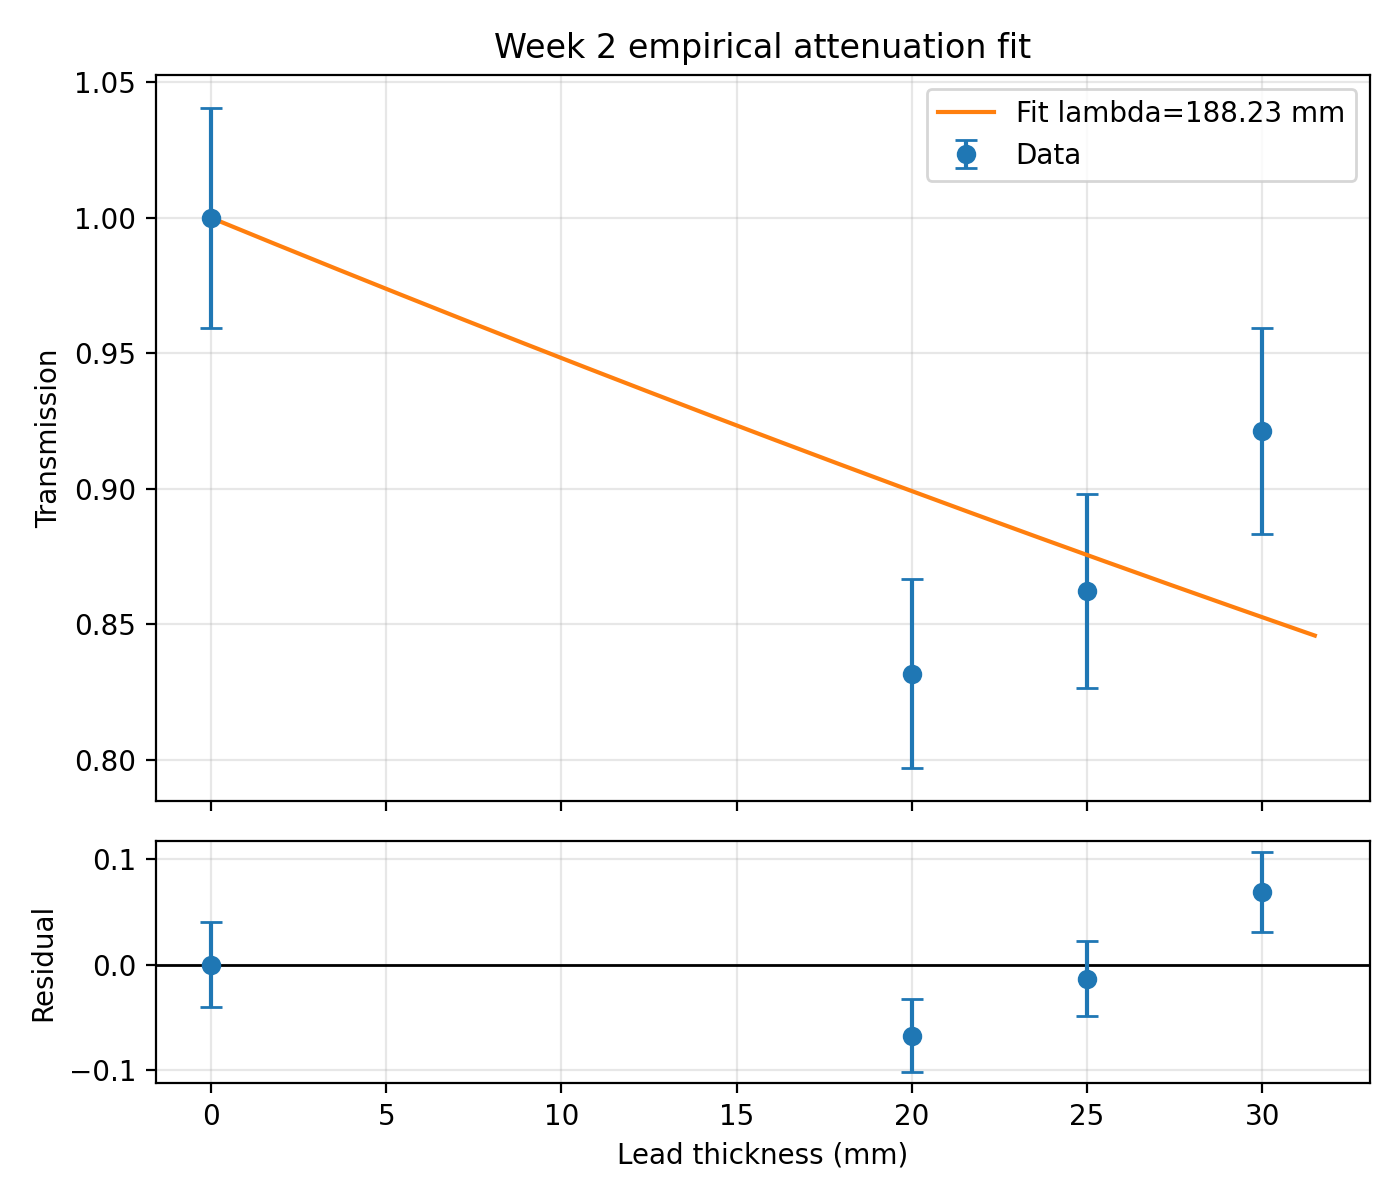
\includegraphics[width=\linewidth]{fit/week2_attenuation_fit.png}
\caption{第二周归一化透过率的经验指数拟合。该拟合只用于展示趋势，不应解释为可靠的铅中衰减长度。}
\label{fig:week2_fit}
\end{figure}

第二周的关键问题在于 0 片基准本身已经不同。如果 0 片数据不能代表与第一周相同的探测器状态，那么用第二周 0 片归一化得到的 40、50、60 片透过率只能描述第二周内部相对变化，而不能直接和第一周的 10、20、30 片点拼接。这一点是后续综合分析的核心限制。

从数据形态看，第二周 40--60 片区间的回升也可能与厚铅板条件下样本组成改变有关，但仅凭当前数据无法把这种物理可能性与探测器系统漂移区分开。因为第二周 0 片基准已经显示下探测器脉冲积分分布明显左移，任何关于厚铅板区间的精细物理解释都必须先经过效率校准。否则，拟合得到的有效衰减长度会把真实铅板作用和探测器状态变化混合在一起。

因此，第二周结果在报告中的主要价值并不是给出更厚铅板下的可靠衰减长度，而是提供一个典型例子：当基准测量发生变化时，归一化和拟合必须谨慎处理。将第二周作为独立数据集讨论，可以避免把非单调趋势误判为铅板物理效应。

第二周 0 片符合数为 1831，显著低于第一周 0 片的 3357。若两周测量时间均约为一小时，则这种差异对应的 counts/hour 变化接近 45\%。这远大于常规泊松涨落：对于 $N\sim3000$ 的计数，$\sqrt{N}/N$ 只有约 2\%。即使加入 1 min 时间误差，也不足以解释如此大的变化。因此，第二周问题不是简单的统计不确定度问题。

第二周厚铅板点的非单调性还会影响拟合参数的物理解释。指数拟合倾向于用一条平滑下降曲线描述所有点，但当数据本身先降后升时，拟合得到的 $\lambda_{\rm eff}$ 会成为折中结果。这样的参数可能在数值上有误差条，却不代表模型假设成立。因此，在论文正文中报告第二周拟合值时，必须同时报告拟合优度和非单调现象，避免给读者造成“第二周也测得了可靠衰减长度”的误解。

\section{跨周一致性分析}

两周 0 片基准符合率差异显著：
\begin{equation}
N_{\rm coin}^{\rm W1}(0)=3357,\qquad
N_{\rm coin}^{\rm W2}(0)=1831.
\end{equation}
第二周 0 片符合率只有第一周的约 $0.545$。这说明两周绝对符合率不能直接拼接。

0 片铅板测量在本实验中承担基准作用。理论上，在没有铅板时，两周若使用相同探测器、相同阈值、相同几何位置和相近环境条件，则 0 片符合率应在统计误差和小幅环境变化范围内接近。现在两周 0 片计数相差接近一半，远大于泊松误差和 1 min 时间误差能够解释的范围，因此必须视为系统性差异。

进一步比较 0 片数据可发现，下探测器响应发生明显变化。第一周 0 片的 $\mathrm{area2}$ 均值为 34.74，而第二周为 17.71。固定阈值 $\mathrm{area2}>30$ 因此在第二周变得更严格，导致下探测器通过率显著降低。

\begin{figure}[h]
\centering
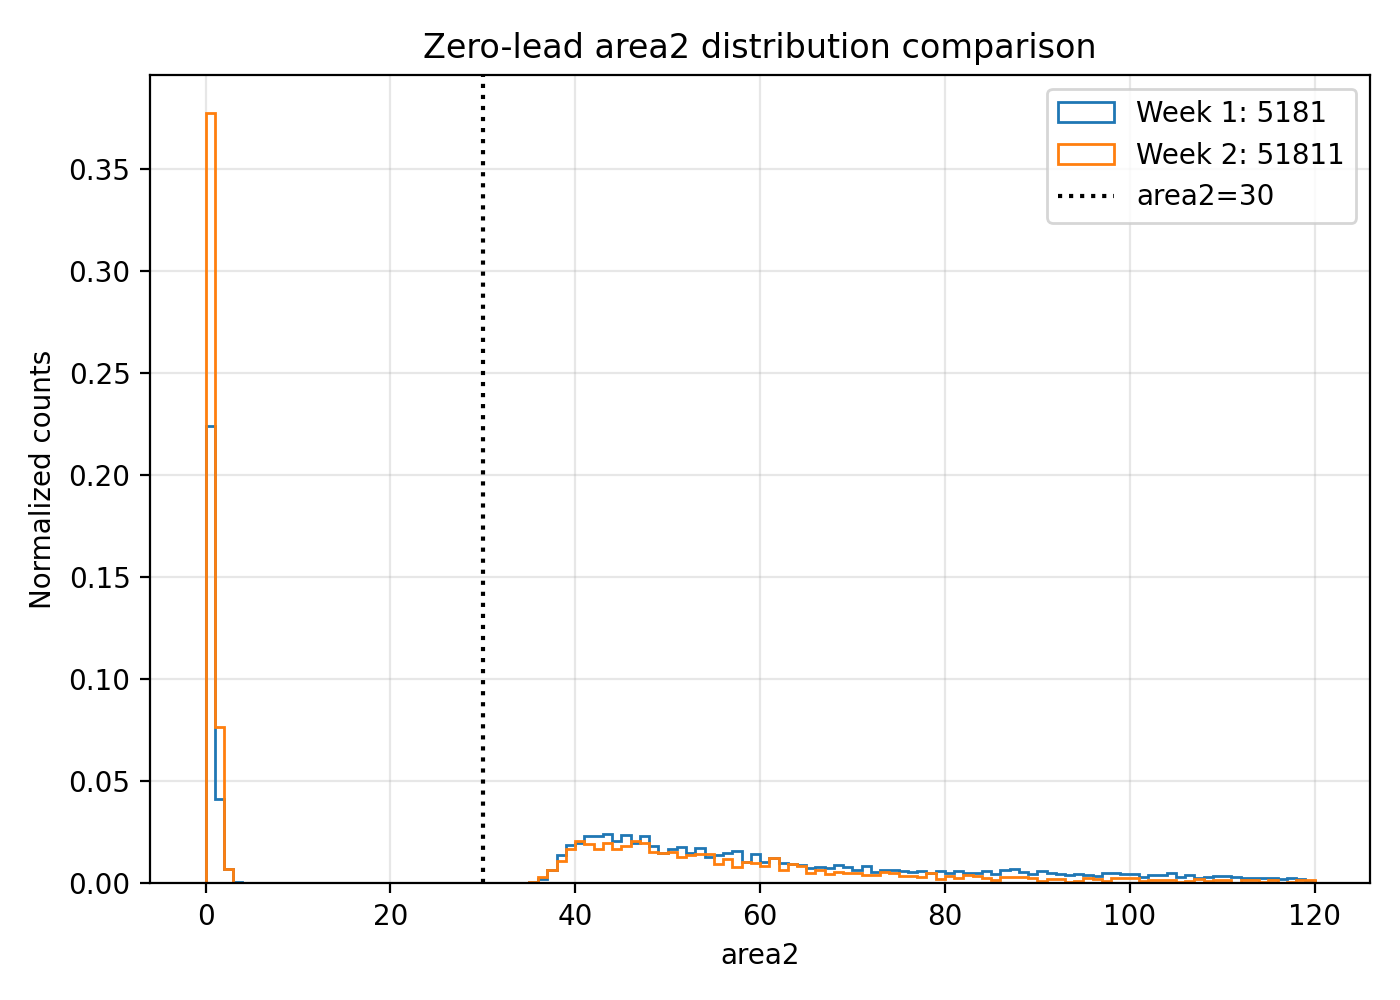
\includegraphics[width=\linewidth]{figures/zero_lead_area2_comparison.png}
\caption{两周 0 片铅板数据的下探测器 \texttt{area2} 分布对比。第二周分布显著左移，说明下探测器响应降低。}
\label{fig:area2_comparison}
\end{figure}

条件符合比也支持这一判断。第一周 0 片数据中 $N_{\rm coin}/N_{\rm up}\approx0.475$，而第二周仅约 0.267。这说明第二周上探测器候选事件形成双探测器符合的概率显著下降。

这一结果具有明确的物理和实验含义。若上探测器计数代表入射候选事件规模，则 $N_{\rm coin}/N_{\rm up}$ 下降意味着许多上探测器事件没有在下探测器形成有效信号。原因可能包括下探测器增益降低、基线或噪声水平变化、阈值相对信号分布的位置改变，也可能包括探测器几何位置或铅板摆放方式的变化。由于 \texttt{area2} 分布整体左移，增益或信号积分尺度变化是最直接的解释。

因此，两周数据的主要差异并不只是宇宙线通量的自然涨落。宇宙线通量在一小时尺度上当然会有统计波动，但不足以解释 0 片符合数和下探测器脉冲积分分布的同步变化。本文把该差异归类为跨周探测效率变化，并在综合分析中通过基准缩放进行一阶修正。

这一判断也解释了为什么跨周分析中不能直接比较绝对 counts/hour。绝对计数率的变化可能来自铅板厚度，也可能来自探测效率，而两者在数学上都表现为计数下降。如果没有 0 片基准和脉冲积分分布的辅助检查，二者很容易混淆。本文把 0 片基准作为“无吸收体时的系统响应标尺”，再利用 \texttt{area2} 分布确认该标尺在两周之间发生改变。

从脉冲积分角度看，固定阈值 $30$ 对第一周和第二周的实际含义并不相同。第一周下探测器 \texttt{area2} 均值约为 34.74，阈值位于分布均值附近；第二周均值约为 17.71，阈值则位于分布较高端。这意味着第二周只有更大脉冲积分事件才能通过下通道选择，导致有效效率降低。这个现象直接解释了为什么第二周条件符合比明显下降。

跨周一致性分析也说明了为什么本报告坚持使用分周讨论。若直接把第二周 40、50、60 片点放在第一周 0、10、20、30 片后面，所得曲线会同时包含铅板厚度效应和探测效率跳变。这样的曲线虽然视觉上覆盖了更宽厚度范围，但物理解释反而更弱。分周讨论能保留每周内部的相对关系，并把跨周差异作为单独问题处理。

\section{跨周归一化}

为了展示 0--60 片铅板的综合趋势，定义 0 片基准缩放因子：
\begin{equation}
k=\frac{R_{\rm coin}^{\rm W1}(0)}{R_{\rm coin}^{\rm W2}(0)}
=\frac{3357}{1831}=1.833.
\end{equation}
第二周缩放后的符合率为
\begin{equation}
R_{\rm coin,scaled}^{\rm W2}(x)=kR_{\rm coin}^{\rm W2}(x).
\end{equation}

该缩放的物理假设是：第二周所有厚度点相对于第一周都受到同一个整体效率因子影响。若这个假设成立，则用 0 片基准确定 $k$ 后，可以把第二周 counts/hour 映射到第一周的探测效率标尺上。换言之，缩放不是改变第二周内部相对透过率，而是把第二周绝对计数率重新放到第一周 0 片基准下比较。

不过这一假设只是近似。若探测器效率变化依赖于脉冲大小、铅板厚度、粒子角度或噪声水平，那么单一 $k$ 无法完全修正所有点。例如，当下探测器 \texttt{area2} 分布靠近阈值时，微小增益变化就可能对通过率产生非线性影响。因此，基准缩放适合展示综合趋势，但不能替代真正的效率校准。

缩放后的 0--60 片趋势见表~\ref{tab:combined}。虽然该方法使两周 0 片基准一致，但第二周厚铅板点仍然不是单调下降，说明单一缩放因子不能完全修正第二周系统效应。

\begin{table}[h]
\caption{0 片基准缩放后的 0--60 片综合趋势。}
\label{tab:combined}
\begin{ruledtabular}
\begin{tabular}{cccc}
Run & 铅板数 & 缩放后 counts/hour & 缩放透过率\\
\hline
5181 & 0  & 3357.0 & 1.000\\
5182 & 10 & 3136.0 & 0.934\\
5183 & 20 & 3119.0 & 0.929\\
5184 & 30 & 3046.0 & 0.907\\
5185 & 40 & 2792.3 & 0.832\\
5186 & 50 & 2895.0 & 0.862\\
5187 & 60 & 3093.0 & 0.921\\
\end{tabular}
\end{ruledtabular}
\end{table}

\begin{figure}[h]
\centering
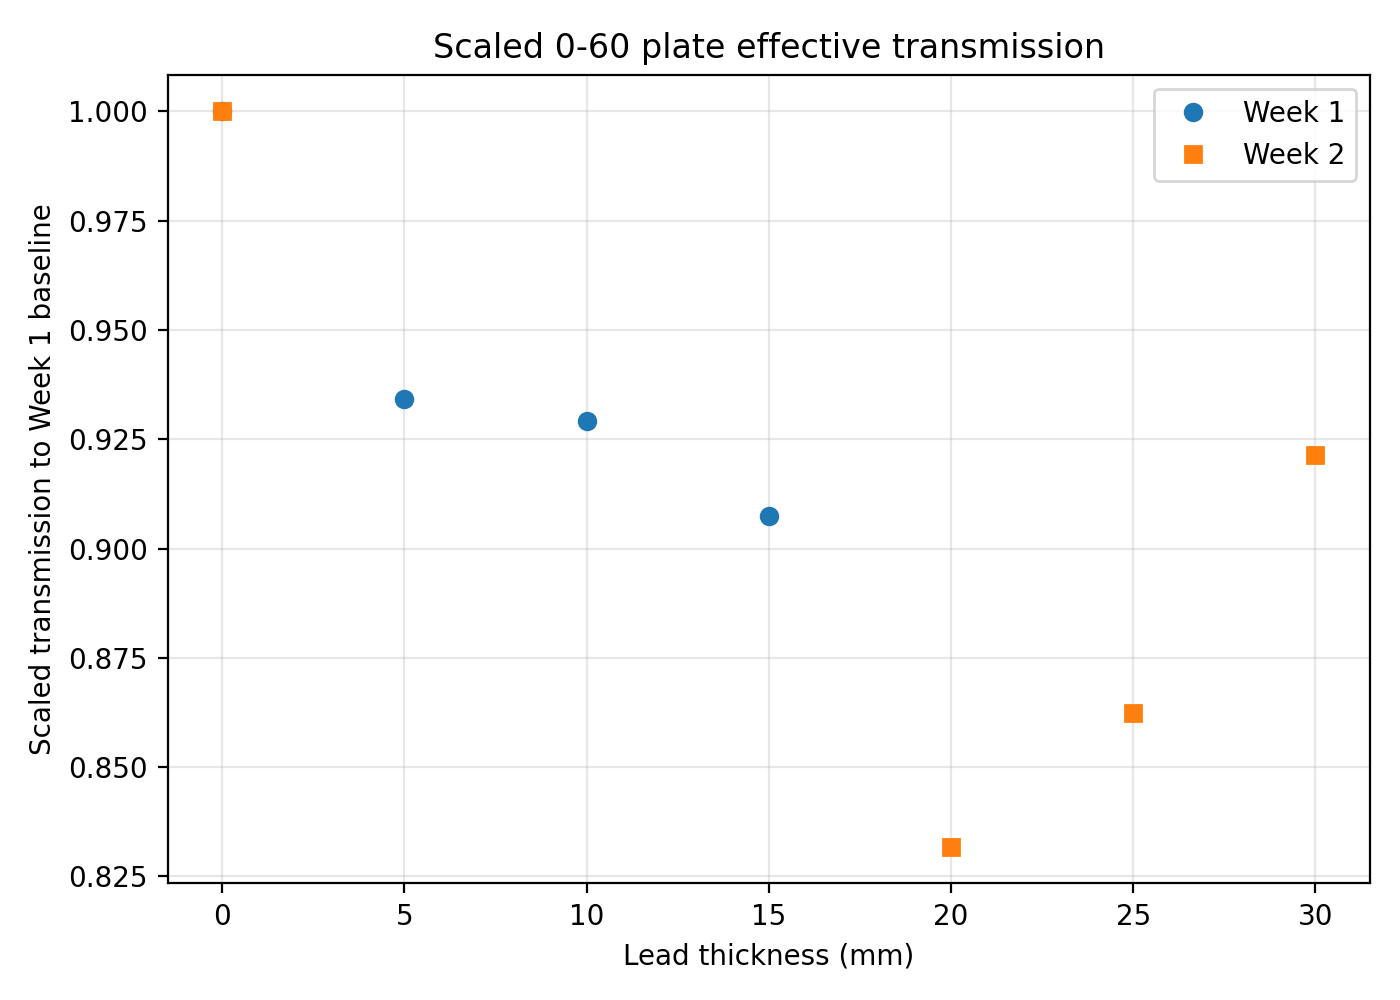
\includegraphics[width=\linewidth]{figures/scaled_transmission_combined.png}
\caption{0 片基准缩放后的 0--60 片有效透过率趋势。第二周厚铅板点仍非单调，表明探测器响应变化尚未被完全修正。}
\label{fig:combined_scaled}
\end{figure}

综合曲线可以给出两个层次的结论。第一，在 0--40 片范围内，缩放后的有效透过率总体从 1 降至约 0.832，说明加入铅板后符合概率确实降低。第二，在 40--60 片范围内，曲线出现回升，因此不能把 0--60 片整体作为严格单调的材料衰减曲线。报告中应明确区分这两层含义：0--40 片的下降趋势支持铅板阻挡能力的定性结论，而 40--60 片的非单调性暴露了系统误差和探测器响应变化。

基准缩放后的 counts/hour 还可以用于直观展示两周数据规模的差别。第二周 40、50、60 片点分别被乘以 $k=1.833$ 后，变为 2792.3、2895.0 和 3093.0 counts/hour。它们低于第一周 0 片点，但 60 片点已经接近第一周 30 片点。这种结果与“铅板越厚符合率越低”的简单预期并不完全一致，进一步说明综合图应作为诊断图，而不是最终的高精度衰减曲线。

如果未来要进行更严格的跨周合并，可以考虑引入效率修正函数而非单一缩放因子。例如可根据下探测器 \texttt{area2} 分布估计固定阈值造成的通过率变化，或者选取分布中更稳定的相对阈值。也可以在每周开始和结束分别测量 0 片数据，检验探测器响应是否随时间连续漂移。当前数据不足以支持这些更复杂修正，因此本文只采用最透明的一阶归一化方法。

缩放后的透过率还可用于估算一个经验阻挡趋势。以第一周 0 片为基准，40 片处有效阻挡率约为 $1-0.832=0.168$，即约 17\%。但 60 片处阻挡率又回到约 8\%。如果只报告 40 片点，会得到铅板阻挡增强的直观结论；如果纳入 50 和 60 片，则必须承认厚铅板区间存在未修正系统效应。因此，综合分析的最终表述应避免给出单一“60 片铅板阻挡率”的强结论。

在图像解释上，综合图的作用是把所有数据放到共同基准下显示，而不是证明所有点服从同一模型。第一周拟合图用于说明薄铅板区间的稳定下降；第二周拟合图用于暴露厚铅板区间的不稳定；0 片 \texttt{area2} 对比图用于证明跨周响应不同；缩放综合图用于展示经过一阶修正后的全厚度范围。这四类图像共同构成本文的证据链。

\section{图像与结果解释}

图~\ref{fig:week1_transmission} 同时给出第一周有效透过率和有效阻挡率。透过率从 1 开始，随铅板厚度增加而下降；阻挡率则从 0 开始，随厚度增加而上升。二者并不是两个独立观测量，而是通过 $\mathcal{B}=1-\mathcal{T}$ 相互定义。将二者画在同一分析中，有助于从“剩余多少符合事件”和“损失多少符合事件”两个角度理解同一组数据。

图~\ref{fig:week1_fit} 展示第一周透过率的指数拟合。该图的主要意义不是证明宇宙线在铅中严格服从单指数吸收，而是给出第一周内部衰减趋势的有效尺度。由于第一周四个点整体下降且拟合优度较好，该图可以作为本文最可靠的物理趋势图。

图~\ref{fig:week2_fit} 展示第二周透过率拟合。与第一周不同，该图应重点观察数据点相对于拟合曲线的偏离，而不是只读取拟合参数。40、50、60 片点出现回升，说明厚铅板区间并未形成稳定单调趋势。因此，该图在报告中的角色是说明第二周存在异常或系统效应。

图~\ref{fig:area2_comparison} 是跨周分析中最重要的诊断图之一。它比较两周 0 片铅板条件下下探测器的脉冲积分分布。由于 0 片时没有铅板影响，若两周探测器状态一致，两条分布应大致接近。实际结果中第二周分布明显左移，说明下探测器响应降低或积分尺度发生变化。这为第二周符合率降低提供了探测器层面的解释。

图~\ref{fig:combined_scaled} 是综合结果图，但它的解释必须最谨慎。该图把第二周 counts/hour 乘以基准缩放因子后，与第一周数据放在同一 0 片标准下比较。它显示 0--40 片范围内存在总体下降，但 40--60 片范围内出现非单调回升。因此，该图不能单独作为铅板衰减规律的证明，而应与跨周诊断图共同使用。

表~\ref{tab:week1}、表~\ref{tab:week2} 和表~\ref{tab:combined} 分别对应三层结果。第一周表格给出最稳定的薄铅板数据；第二周表格给出厚铅板数据及其非单调特征；综合表格给出缩放后的全厚度范围。三张表的顺序体现了本文的分析逻辑：先建立可靠局部趋势，再识别跨周问题，最后给出带有限制条件的综合趋势。

在最终论文写作中，图像说明应避免只重复坐标轴内容，而要指出图像支持了哪一个物理判断。例如，第一周透过率图支持铅板降低有效符合率；第二周拟合图支持厚铅板区间存在异常；0 片脉冲积分图支持跨周探测器响应漂移；综合缩放图支持一阶归一化可以展示全范围趋势但不能完全修正系统误差。

\section{误差与系统效应}

本实验误差分析的核心是区分随机误差和系统误差。随机误差来自有限计数，主要服从泊松分布。对于符合数 $N_{\rm coin}$，标准差近似为 $\sqrt{N_{\rm coin}}$。当 $N_{\rm coin}$ 在 $10^3$ 量级时，统计相对误差为几个百分点。因此，若相邻厚度点只相差几十个计数，就不能赋予过强物理解释；若整体变化达到数百个计数，则更可能反映真实趋势或系统变化。

测量时间误差也是本实验的显式误差来源。每个 run 取一小时，误差估计为 1 min，因此相对时间误差为
\begin{equation}
\frac{\sigma_T}{T}=\frac{60}{3600}=0.0167.
\end{equation}
这个误差会直接传递到计数率 $R=N/T$ 中。由于不同厚度点测量时间相同，时间误差对绝对 counts/hour 拟合和相对透过率拟合的影响略有不同；在透过率中，若各 run 时间误差独立，则仍会贡献相对不确定度。

系统误差比随机误差更难量化。固定阈值是最重要的系统来源之一。阈值 $30$ 的选择在第一周可能处于较合理的信号区间，但在第二周下探测器响应降低后，该阈值变成更强的筛选条件。于是同样的物理粒子在两周中可能得到不同的通过概率。这类误差不会通过增加计数时间自动消失，必须通过标定、效率修正或重复基准测量控制。

几何误差也会影响符合率。上下探测器的相对位置、铅板是否水平、铅板是否完全覆盖有效区域，都会改变粒子穿过两探测器的几何接受度。对于多重散射问题，探测器间距越大，给定散射角造成的横向偏移越明显。因此，如果两周铅板堆叠位置或探测器相对位置发生变化，厚铅板点的符合率可能受到额外影响。

环境因素也可能造成较小影响。大气压变化会改变宇宙线到达地面的通量，温度变化可能影响 SiPM 增益和电子学响应。对于精密宇宙线实验，这些因素需要用气象数据和探测器温度记录修正。当前课程实验缺少这些外部记录，因此本文只在系统误差讨论中定性指出其可能性，不对其进行数值修正。

综合来看，第一周主要受随机误差和较小系统误差影响，第二周则明显受探测器响应系统变化影响。这个判断决定了本文结果的权重分配：第一周可以作为主要物理趋势依据，第二周主要用于讨论跨周一致性和厚铅板区间的不确定性，综合缩放结果作为辅助展示。


\section{讨论}

第一周数据在内部具有较好一致性，符合率随铅板厚度增加整体下降。该趋势可以用有效衰减模型描述，但其物理含义应理解为几何、阈值和探测效率条件下的有效符合概率衰减。

第二周数据则表现出明显系统效应。0 片基准符合率显著低于第一周，下探测器 \texttt{area2} 分布明显左移，条件符合比也发生显著变化。这些现象说明第二周探测系统响应发生了变化，尤其是下探测器通道可能存在增益或阈值效率变化。

因此，跨周综合结果应谨慎解释。0 片基准缩放可以展示一个形式上的 0--60 片趋势，但不能完全消除系统误差。更稳妥的做法是分别报告两周内部结果，并将跨周归一化差异作为系统误差讨论。

本实验中“阻挡能力”的检测并不是直接测量铅板吸收了多少 $\mu$ 子，而是测量加入铅板后双探测器有效符合率下降了多少。因此，当我们说铅板具有阻挡作用时，实际含义是铅板降低了满足本实验符合条件的事件比例。这个比例包含真实低能成分损失、散射导致的几何损失以及阈值响应造成的效率损失。对于教学实验而言，这种定义是合理的，因为探测器最终记录的就是符合事件，而非入射粒子的完整相空间信息。

误差来源可以分为统计误差和系统误差。统计误差主要来自有限计数的泊松涨落，随 $1/\sqrt{N}$ 缩小。时间误差来自测量时间约 1 min 的不确定度。系统误差则包括阈值选择、通道增益漂移、基线变化、探测器相对位置变化、铅板摆放不完全一致以及宇宙线环境变化等。在本数据中，系统误差显然占据重要地位，尤其是第二周下探测器响应变化。

若要改进实验，可在每次改变铅板厚度前后重复测量 0 片基准，以监控探测器效率漂移；也可记录更长时间以降低统计误差；还可对上下探测器分别进行脉冲积分标定，使阈值以相对信号尺度而非固定 ADC 积分值定义。若能够获得探测器间距和有效面积，还可以进一步估算几何接受度，并把多重散射导致的偏离概率与实验符合率联系起来。

本文暂不讨论 Rossi 曲线的完整测量。Rossi 曲线通常关注宇宙线在吸收体中产生二次粒子后计数率随吸收体厚度的先升后降行为，需要更系统的厚度扫描和稳定探测条件。当前数据的重点是铅板厚度对双探测器有效符合率的影响，以及两周探测效率变化对合并分析的限制。

指数模型在本文中也有明显局限。真实宇宙线样本由不同能量和角度的粒子组成，每一类粒子在铅中的散射和能损不同，叠加后未必严格服从单指数形式。双探测器几何还会把角度变化转化为符合效率变化，使 $\lambda_{\rm eff}$ 同时包含材料和装置因素。因此，$\lambda_{\rm eff}$ 更适合作为不同数据集之间的经验比较参数，而不是与文献中的材料吸收长度逐项对比。

尽管存在这些限制，本实验仍然给出了清楚的物理图像：铅板会降低有效符合事件数，而探测器响应稳定性决定了这种降低能否被可靠量化。第一周数据展示了较一致的厚度依赖；第二周数据提醒我们，任何探测器实验都必须用基准点和分布诊断来监控效率。对于课程实验报告而言，这一点本身就是重要结论。

\section{结论}

本文完成了宇宙线铅板阻挡实验的分周和综合分析。第一周结果显示，铅板厚度从 0 增加到 15 mm 时，双探测器有效符合率整体下降，并给出约 $10^2$ mm 量级的有效衰减长度。第二周厚铅板数据存在非单调趋势和明显探测器响应漂移，不能作为干净的铅板衰减曲线解释。跨周 0 片基准缩放后可得到 0--60 片的综合趋势，但厚铅板区间仍显示系统效应。因此，本实验测量的是有效符合率衰减，而不是 $\mu$ 子在铅中的纯吸收长度。

从实验报告的最终表述看，最稳妥的结论是：第一周数据支持铅板增加会降低双探测器有效符合率；第二周数据揭示了探测器响应变化对符合测量的显著影响；跨周归一化可以作为展示综合趋势的一阶方法，但不能完全修正系统误差。该实验展示了宇宙线穿过物质后的计数率变化，也说明了在实际探测器实验中，效率校准和基准测量与物理模型本身同样重要。

\begin{thebibliography}{99}

\bibitem{pdg_cosmic}
Particle Data Group, ``Cosmic Rays,'' \textit{Review of Particle Physics} (2024).

\bibitem{pdg_matter}
Particle Data Group, ``Passage of Particles Through Matter,'' \textit{Review of Particle Physics} (2024).

\bibitem{rossi1933}
B. Rossi, ``Interaction between Cosmic Rays and Matter,'' \textit{Nature} \textbf{132}, 173 (1933).

\bibitem{rossi_book}
B. Rossi, \textit{High-Energy Particles} (Prentice-Hall, 1952).

\bibitem{caen}
CAEN, ``DT5742 Digitizer Documentation,'' \url{https://www.caen.it/products/dt5742/}.

\end{thebibliography}

\end{document}
